\runningheader{SAT Mathematics}{Drill Set 11}{Page \thepage\ of \numpages}

\begingradingrange{sat-drill-11}
\subsection*{SAT Drill 11}

\question[1]
The value of a new boat depreciates at a rate of $12\%$ per year. The function $h(t) = 80,000\left(1-\frac{12}{100}\right)^t$ gives the value of the boat, in dollars, after $t$ years. Which of the following expressions could be used to determine the number of years it would take for the value of the boat to decrease by $25\%$?
\begin{choices}
  \choice $20,000 = 80,000\left(1-\frac{12}{100}\right)^t$
  \choice $20,000 = 80,000\left(1-\frac{25}{100}\right)^t$
  \CorrectChoice $60,000 = 80,000\left(1-\frac{12}{100}\right)^t$
  \choice $60,000 = 80,000\left(1-\frac{12}{100}\right)^{4t}$
\end{choices}

\question[1]
Consider the system of equations:
\[
  \begin{gathered}
  2x + 3y = 12 \\
  y = -\frac{2}{3}x + 12
  \end{gathered}
\]
At how many points do the graphs of the given equations intersect in the $xy$-plane?
\begin{choices}
  \CorrectChoice Zero
  \choice Exactly one
  \choice Exactly two
  \choice Infinitely many
\end{choices}

\question[1]
A partially filled gas tank contains 2 gallons of gasoline. If a fuel pump can pump at 0.5 gallons per second and the maximum capacity of the tank is 14 gallons, after how much time, in seconds, will the tank be full?
\begin{solution}
24
\end{solution}



\newpage



\question[1]
From 1994 to 1995, the amount of money, in dollars, a company made grew by $6\%$. Each year for the next ten years, the amount of money the company made increases by the amount earned between 1994 and 1995. What type of function best models the relationship between the money the company made, in dollars, and time, in years?
\begin{choices}
  \choice Decreasing linear
  \choice Decreasing exponential
  \CorrectChoice Increasing linear
  \choice Increasing exponential
\end{choices}

\question[1]
If $\frac{p}{q}=\frac{4}{3}$, what is the value of $\frac{12q}{p}$?
\begin{choices}
  \choice 6
  \choice 8
  \CorrectChoice 9
  \choice 16
\end{choices}

\question[1]
What is the sum of all values of $b$ that satisfy the equation $3b^2-2b-4=0$?
\begin{choices}
  \CorrectChoice $\frac{2}{3}$
  \choice $\frac{3}{2}$
  \choice $\frac{\sqrt{13}}{3}$
  \choice $2\sqrt{13}$
\end{choices}

\question[1]
Let $f(x) = m x + 4$ and $g(x) = \frac{1}{2}x - 5$. If $f(2) = g(4)$, what is the value of $m$?
\begin{choices}
  \choice $-4$
  \CorrectChoice $-3.5$
  \choice $-3$
  \choice $-2$
\end{choices}

\newpage

\question[1]
Triangles $ABC$ and $XYZ$ are shown in the figure below (not drawn to scale). If $\frac{AB}{BC}=k$, where $k$ is a constant, which of the following ratios is equal to $k$?
\begin{center}
  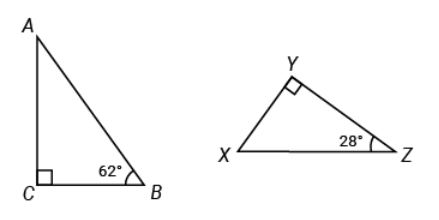
\includegraphics[width=0.90\linewidth]{images/cus24}
\end{center}
\begin{choices}
  \choice $\frac{XZ}{XY}$
  \choice $\frac{XY}{XZ}$
  \choice $\frac{YZ}{XZ}$
  \choice $\frac{XZ}{YZ}$
\end{choices}

\question[1]
Let $f(x) = -200(3)^x$ and $g(x) = -200(3)^{x+a}$, where $a$ is a positive constant. Which of the following statements about the functions $f$ and $g$ must be true?
\statementbox{
  \begin{enumerate}[label=(\Roman*)]
    \item The $y$-intercept of the graph of $g$ is less than the $y$-intercept of the graph of $f$.
    \item The $y$-intercept of the graph of $g$ is greater than the $y$-intercept of the graph of $f$.
    \item If $a < b$, then $f(a) < f(b)$.
  \end{enumerate}
}
\begin{choices}
  \CorrectChoice I only
  \choice II only
  \choice I and III only
  \choice II and III only
\end{choices}



\newpage



\question[1]
If $(a x + 4)(3 x + b) = 18 x^2 + c x + 12$ for all $x$, what is the value of $c$?
\begin{choices}
  \choice 3
  \choice 6
  \choice 15
  \CorrectChoice 30
\end{choices}

\question[1]
The equation $x^2 + y^2 = 4x - 6y + 23$ defines a circle in the $xy$-plane. What is the length of the radius of the circle?
\begin{solution}
6
\end{solution}

\question[1]
If $x^3 - 7x^2 + 3x - 21 = 0$, what is a real number solution for $x$?
\begin{solution}
7
\end{solution}

\question[1]
Square $ABCD$ has an area of 100 square units. If $E, F, G,$ and $H$ are all midpoints of the sides of $ABCD$, respectively, what is the perimeter, in units, of square $EFGH$?
\begin{choices}
  \choice $5\sqrt{2}$
  \choice 20
  \CorrectChoice $20\sqrt{2}$
  \choice $40\sqrt{2}$
\end{choices}



\newpage



\question[1]
Let $h(x) = \frac{1}{(x+3)^2 + (x+3) - 42}$. For what value of $x > 0$ is the function $h(x)$ undefined?
\begin{solution}
3
\end{solution}

\question[1]
The variables $x$ and $y$ are related such that each time $x$ increases by 4, $y$ decreases by 3. If the function goes through the point $(8, -5)$, which of the equations below represents the function?
\begin{choices}
  \choice $3x + 4y = -5$
  \choice $4x - 3y = 1$
  \choice $4x - 3y = 8$
  \CorrectChoice $3x + 4y = 4$
\end{choices}

\question[1]
Line $m$ passes through the points $(a, 0)$ and $(0, c)$, where $a$ and $c$ are real numbers that do not equal 0. If line $n$ is perpendicular to line $m$ and the lines intersect at $(0, c)$, what is the equation of line $n$?
\begin{choices}
  \choice $y = -\frac{a}{c}x + c$
  \choice $y = -\frac{c}{a}x + c$
  \CorrectChoice $y = \frac{a}{c}x + c$
  \choice $y = \frac{c}{a}x + c$
\end{choices}





\newpage




\question[1]
Which of the following inequalities represents the shaded region in the given graph?
\begin{center}
  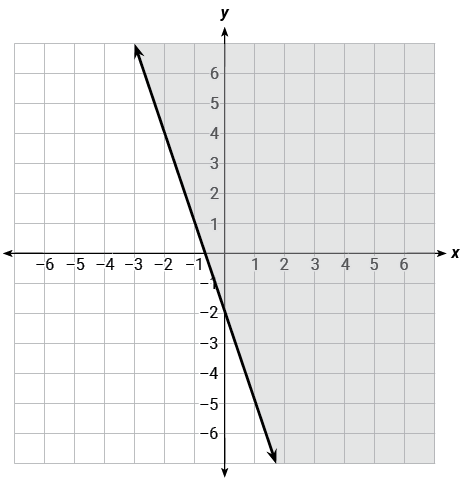
\includegraphics[width=0.90\linewidth]{images/cus25}
\end{center}
\begin{choices}
  \choice $y \leq -2x - 2$
  \choice $y \leq -3x - 2$
  \choice $y \geq -2x - 2$
  \choice $y \geq -3x - 2$
\end{choices}

\question[1]
Let $f(x) = mx + b$ and $g(x) = 2x^2 - 8x + 13$. In the given system, $m$ and $b$ are constants, $f(x)$ intersects $g(x)$ at the minimum of $g(x)$, and the functions have the same $y$-intercept. What is the value of $m$?
\begin{choices}
  \CorrectChoice $-4$
  \choice $-2$
  \choice 5
  \choice 13
\end{choices}


\newpage




\question[1]
Mr. Kim collected the homework from his students and made a graph to show how many problems his students were able to complete. One of his students turned in their homework late and they completed 10 problems. Which of the following describes what will happen to the data when that data point is added?
\begin{center}
  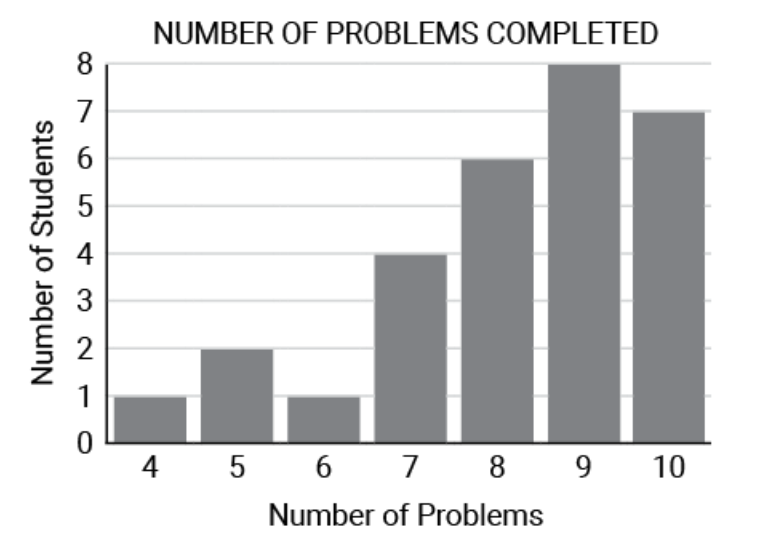
\includegraphics[width=0.90\linewidth]{images/cus26}
\end{center}
\begin{choices}
  \choice The mean and median will not change.
  \choice The mean will increase slightly and the median will not change.
  \choice The mean will not change and the median will increase slightly.
  \choice The mean and median will increase slightly.
\end{choices}

\question[1]
A circle graphed on the coordinate plane is centered at the origin, labeled point $O$. Point $X$ lies on the circle at $(-k, k\sqrt{3})$. Point $Y$ lies on the circle at $(-2k, 0)$. Which of the following is the measure of angle $XOY$?
\begin{choices}
  \choice $\frac{\pi}{6}$
  \CorrectChoice $\frac{\pi}{3}$
  \choice $\frac{2\pi}{3}$
  \choice $\frac{5\pi}{6}$
\end{choices}



\newpage




\question[1]
The force of gravity on Earth is 9.8 meters per second squared. The gravitational force on Mars is $62\%$ less than that on Earth. What is the approximate force of gravity on Mars, in kilometers per minute squared?
\begin{choices}
  \choice 0.22
  \choice 0.36
  \CorrectChoice 13.41
  \choice 21.87
\end{choices}

\question[1]
$A$ is the first of six consecutive odd integers. If the product of 12 and the 3rd integer is at most 18 less than the sum of the 4th and 6th integers, what is the greatest value of $A$?
\begin{choices}
  \choice $-6$
  \CorrectChoice $-5$
  \choice 3
  \choice 11
\end{choices}

\question[1]
Consider the system:
\[
  \begin{gathered}
  4x + 2y = k \\
  y = x^2 - 2x - 3
  \end{gathered}
\]
At what value of $k$ will the system of equations have exactly one real solution?
\begin{choices}
  \CorrectChoice $-6$
  \choice $-3$
  \choice $0$
  \choice $12$
\end{choices}



\newpage




\question[1]
Consider the equation:
\[
  5(x+3) - 3(2-x) = p x + 7
\]
In the given equation, $p$ is a constant. If the equation has no solution, what is the value of $p$?
\begin{solution}
8
\end{solution}

\question[1]
An antique grandfather clock chimes every hour. At one o'clock it chimes once, at two o'clock it chimes twice, and so on. Each chime rings for 1 second, and there are 3 seconds between each chime. At 8 pm, how many seconds does it take from the start of the first chime to the end of the last one?
\begin{solution}
29
\end{solution}

\question[1]
The function $f(T) = \frac{9}{5}T + 32$ determines the temperature in Fahrenheit, where $T$ represents the temperature in degrees Celsius. At what temperature, in degrees, is the Celsius temperature the same as the Fahrenheit temperature?
\begin{choices}
  \CorrectChoice $-40$
  \choice $-17.8$
  \choice $0$
  \choice $32$
\end{choices}



\newpage




\question[1]
A bag of candy contains a certain percentage of chocolate bars. Of the chocolate bars, $25\%$ are white chocolate. If $20\%$ of the candy in the bag is white chocolate bars, what percentage of the candy is chocolate bars?
\begin{choices}
  \choice $20\%$
  \choice $45\%$
  \choice $60\%$
  \CorrectChoice $80\%$
\end{choices}

\question[1]
The perimeter of a rectangle is 72 feet. If the length is twice the width, what is the area of the rectangle, in square feet?
\begin{solution}
288
\end{solution}

\question[1]
The equation $(x-4)^2 + (y+6)^2 = 576$ represents a circle in the $xy$-plane. What is the distance between the center of the circle and the point on the circle with the greatest value of $y$?
\begin{solution}
24
\end{solution}



\newpage




\question[1]
In a data set, the mean is 10, the median is 10, the middle three values are 10, and the largest value is greater than 10. If the largest value is removed from the data set, which of the following correctly represents the changes to the mean and median?
\begin{choices}
  \choice The mean will decrease and the median will decrease.
  \CorrectChoice The mean will decrease and the median will stay the same.
  \choice The mean will increase and the median will stay the same.
  \choice The mean will stay the same and the median will stay the same.
\end{choices}

\question[1]
Triangle $A$ and triangle $B$ are similar right triangles. The hypotenuse of triangle $A$ is 13 inches, and the hypotenuse of triangle $B$ is 26 inches. If the area of triangle $A$ is 30 square inches, what is the area of triangle $B$, in square inches?
\begin{choices}
  \choice 60
  \CorrectChoice 120
  \choice 180
  \choice 240
\end{choices}

\question[1]
For the function $f(x) = a x + b$, $f(-4) = 6$ and $f(8) = 9$. What is the value of $a + b$?
\begin{solution}
$\frac{29}{4}$
\end{solution}



\newpage




\question[1]
How many distinct real solutions does the given equation have?
\[
  9(2x+3) - 10(x+1) = 12(x-1) - 2(2x+5)
\]
\begin{choices}
  \CorrectChoice Zero
  \choice Exactly one
  \choice Exactly two
  \choice Infinitely many
\end{choices}

\question[1]
A line with the equation $12x - 5y = 30$ passes through the points $(0, p)$ and $(q, 0)$. What is the value of $\frac{q}{p}$?
\begin{choices}
  \choice $-\frac{12}{5}$
  \CorrectChoice $-\frac{5}{12}$
  \choice $\frac{5}{12}$
  \choice $\frac{12}{5}$
\end{choices}

\question[1]
The expression $\frac{(x+2)(x^2-3x-28)}{x-7}$ is equivalent to $x^2 + 2a x + 2b$. What is the value of $a + b$?
\begin{solution}
7
\end{solution}

\question[1]
The equation $|3x-4| = x+12$ has two solutions, $p$ and $q$. What is the value of $pq$?
\begin{choices}
  \CorrectChoice $-16$
  \choice $8$
  \choice $16$
  \choice $64$
\end{choices}

\question[1]
For the function $f(x) = a^x + b$, where $a > 0$, $f(1) = 12$ and $f(2) = 24$. What is the value of $b$?
\begin{solution}
8
\end{solution}

\question[1]
The gravity on Mercury is $3.7\,\frac{m}{s^2}$. Which of the following is equal to the gravity on Mercury in kilometers per hour squared, or $\frac{km}{h^2}$? (1 kilometer $= 1,000$ meters)
\begin{choices}
  \choice 13.32
  \choice 1,027.8
  \choice 1,332
  \CorrectChoice 47,952
\end{choices}

\question[1]
Given the linear function $f(x) = a x + b$ and the quadratic function $g(x) = a x^2 + b x$, what are the values of $x$ at which $f(x) = g(x)$?
\begin{choices}
  \choice $x = -1$ and $x = \frac{-a}{b}$
  \choice $x = -1$ and $x = \frac{-b}{a}$
  \choice $x = 1$ and $x = \frac{-a}{b}$
  \CorrectChoice $x = 1$ and $x = \frac{-b}{a}$
\end{choices}



\newpage




\question[1]
The height, in meters, of a projectile launched from a cliff after $t$ seconds can be modeled by the function $h(t) = -4.9 t^2 + 19.6 t + 58.8$. What is the maximum height, in meters, the projectile will reach?
\begin{choices}
  \choice 2
  \choice 58.8
  \CorrectChoice 78.4
  \choice 83.3
\end{choices}

\question[1]
In the figure, the measure of $\angle 1 = a^\circ$, the measure of $\angle 3 = b^\circ$, and the measure of $\angle 5 = c^\circ$. What is the sum of the measure of $\angle 2$ and the measure of $\angle 4$, in degrees?
\begin{center}
  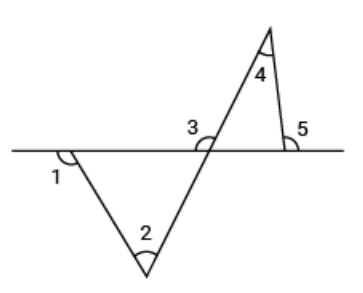
\includegraphics[width=0.90\linewidth]{images/cus27}
\end{center}
\begin{choices}
  \choice $a + b + c - 180$
  \choice $a + 2b + c - 180$
  \choice $a + b + c - 360$
  \choice $a + 2b + c - 360$
\end{choices}




\newpage





\question[1]
In the $xy$-plane, a parabola has a vertex of $(3, -10)$ and intersects the $x$-axis at two points. If the equation of the parabola is in the form $y = a x^2 + b x + c$, where $a, b, c$ are constants, which of the following could be the value of $a + b + c$?
\begin{choices}
  \CorrectChoice $-6$
  \choice $-10$
  \choice $-12$
  \choice $-14$
\end{choices}

\question[1]
Researchers studying the bee population in Epsilon Park divided the park into 21 sections of identical areas and recorded how many bee hives were found in each sector. The results are shown in the dot plot. If the sector that had 5 bee hives was removed from the data, which of the following statements is true?
\begin{center}
  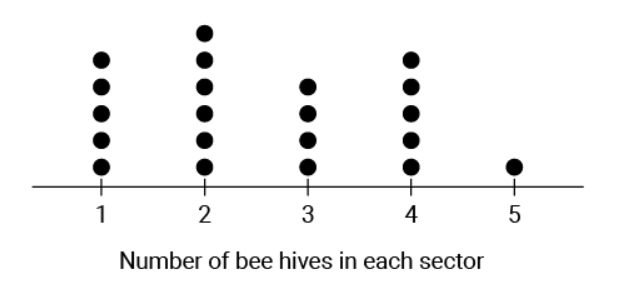
\includegraphics[width=0.90\linewidth]{images/cus28}
\end{center}
\begin{choices}
  \choice The median and mean will decrease.
  \choice The median and mean will stay the same.
  \choice The median will decrease and the mean will stay the same.
  \choice The median will stay the same and the mean will decrease.
\end{choices}



\newpage




\question[1]
Consider the equation $x^2 + qx + p = 0$, where $p$ and $q$ are positive integer constants. If the equation has two distinct integer solutions and $p$ is a prime number, what is the value of $q$?
\begin{choices}
  \choice $2p$
  \choice $\sqrt{p}$
  \choice $p-1$
  \CorrectChoice $p+1$
\end{choices}

\endgradingrange{sat-drill-11}
